Plusieurs pièces mécaniques ont dû être développées pendant ce projet comme par exemple le support de pieds  qui a déjà été décrit au chapitre \ref{sec:DescStruct}.
Maintenant que les éléments sont en place, il faut les lier ensemble avec des pièces faites sur mesure. Toutes les pièces sont faîtes
d'aluminium EN-AW 6082 sauf si mentionné autrement.

\section{Liaison Moteur-Glider}\label{sec:LiaisonMotGlid}
La liaison entre le chariot du guidage et le \gls{glider} du moteur va se faire en deux pièces vissées ensemble. La pièce
connectée au chariot devra accueillir deux roulements qui servent à faire tourner la partie qui tient la tige du pendule. Une zone pour placer
un anneau de LEDs est aussi nécessaire afin de pouvoir illuminer la tige. Enfin, cette pièce devra aussi accueillir l'encodeur pour la position
angulaire. La fixation sur le chariot se fait avec quatre vis M5 ce qui nécessitera donc des lamages. La fixation sur l'autre pièce se fait sur
le dessous de la pièce avec quatre taraudages M5. Un rebord pour l'indexage avec l'autre pièce est aussi présent. On obtient la pièce suivante.

\begin{figure}[H]
  \centering
  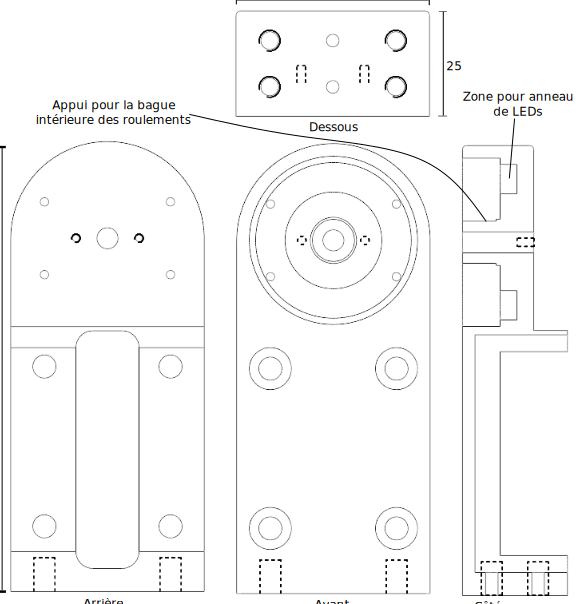
\includegraphics[width = 0.4\textwidth]{assets/figures/LiaisonChariot.png}
  \caption{Représentation de la pièce de liaison du chariot}
  \label{fig:LiaisonChariot}
\end{figure}

La seconde pièce devra évidemment se lier avec la première, mais aussi avec le moteur. La première pièce ayant les taraudages, celle-ci aura quatre
lamages M5. Pour la fixation au moteur, quatre lamages M3 suffiront. Deux autres éléments viennent encore se fixer sur cette pièce: le support de
la tête de lecture pour la règle linéaire et la chaîne porte-câbles. Pour le support de tête de lecture, trois taraudages M4 sont placés sur un côté,
alors que deux trous taraudés sont utilisés pour fixer la chaîne porte-câbles. Finalement, voilà à quoi ressemble la pièce.

\begin{figure}[H]
  \centering
  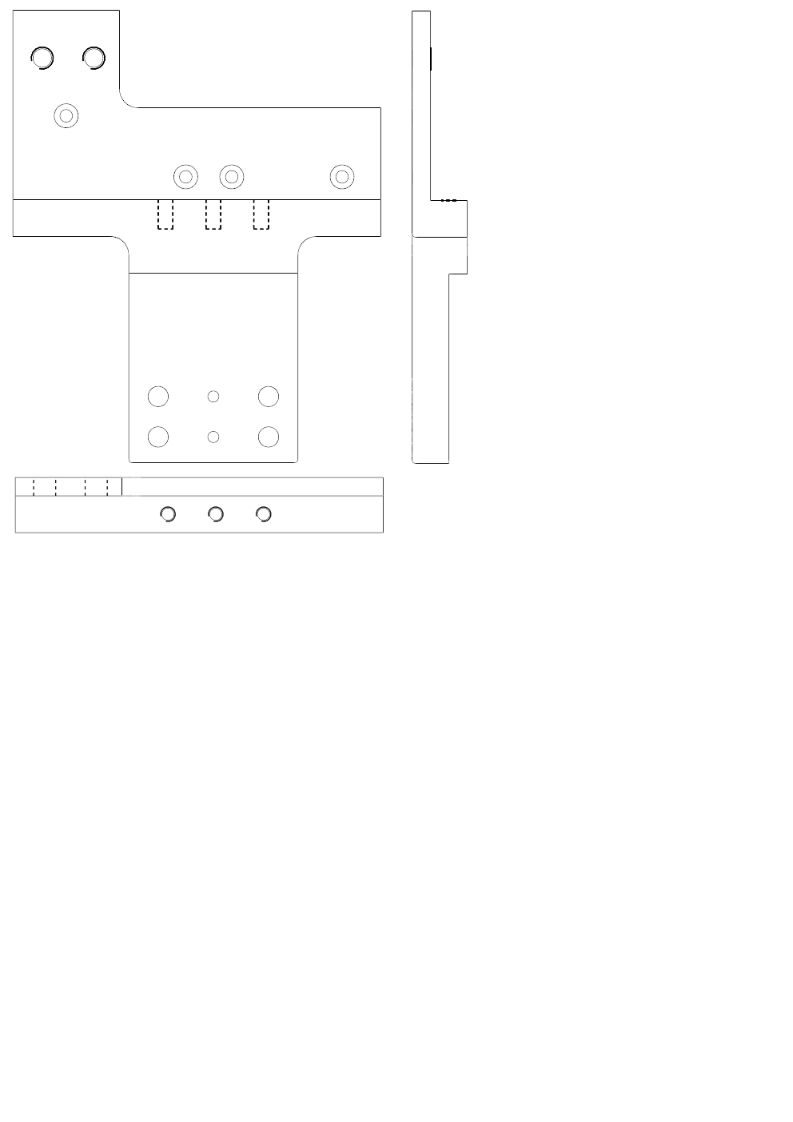
\includegraphics[width = 0.4\textwidth]{assets/figures/LiaisonMoteur.png}
  \caption{Représentation de la pièce de liaison du moteur}
  \label{fig:LiaisonMoteur}
\end{figure}

L'assemblage de ces pièces entre elles et avec leur liaisons directes donne la représentation suivante.

\begin{figure}[H]
  \centering
  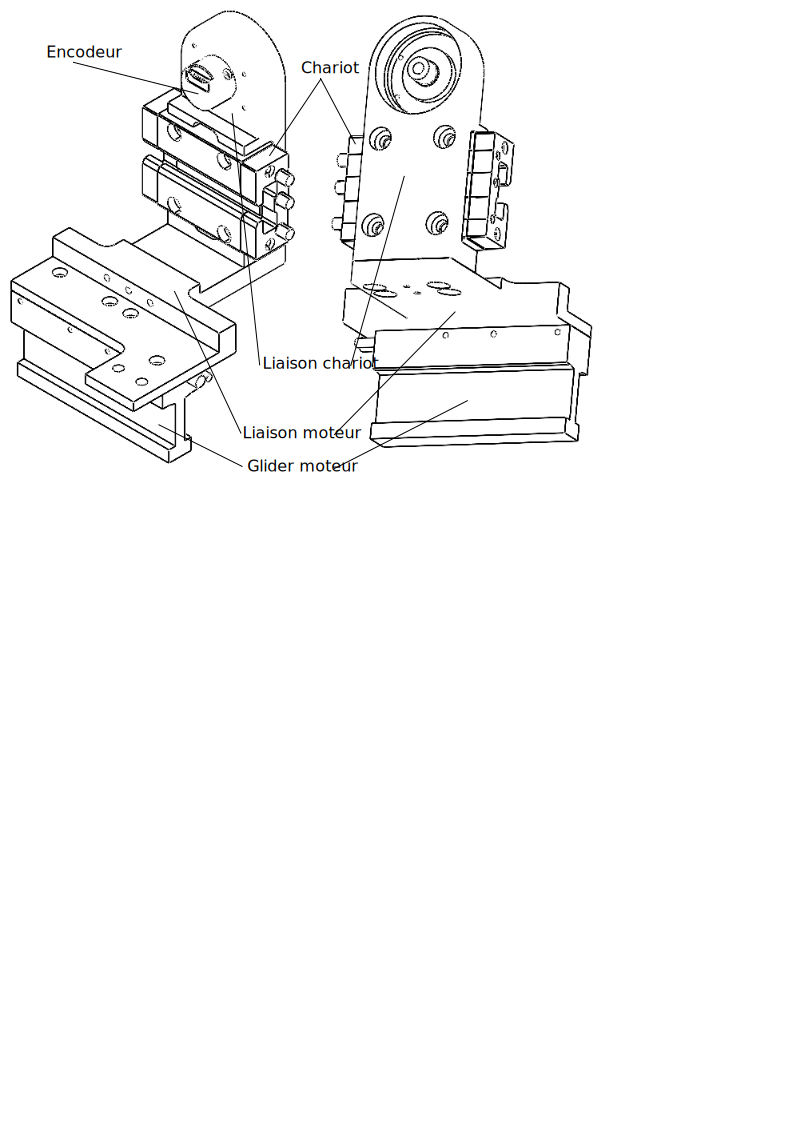
\includegraphics[width = 0.8\textwidth]{assets/figures/AssemblageGuidageEntrainement.png}
  \caption{Représentation de l'assemblage des pièces de guidage et d'entrainement du système}
  \label{fig:AssGuiEntr}
\end{figure}

\section{Support tête de lecture}\label{sec:SupTeteLect}
Le support de la tête de lecture de la règle linéaire est fixé sur la pièce attachée au moteur comme mentionné plus haut. Elle aura donc trois
lamages M4 pour se fixer à la liaison moteur et aussi deux trous de passage pour vis M3 pour la tête de lecture. Un trou supplémentaire est ajouté
pour faire le réglage en position de la tête. La pièce obtenue est la suivante.

\begin{figure}[H]
  \centering
  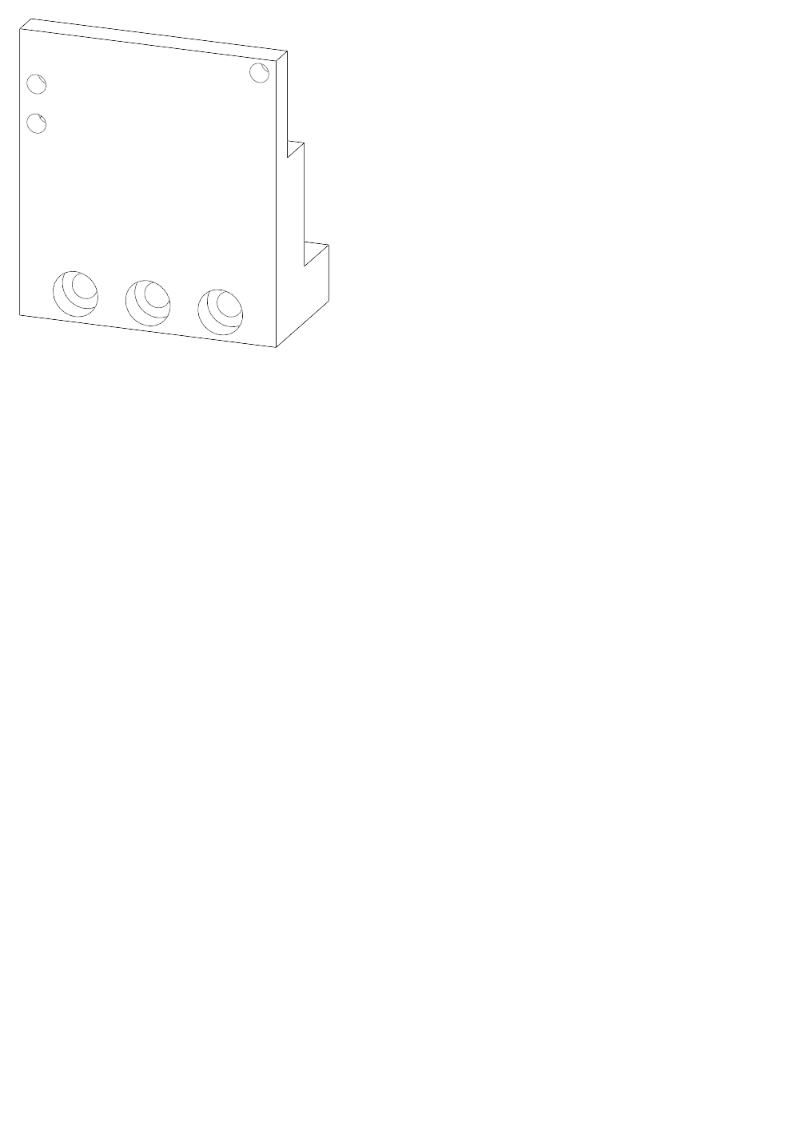
\includegraphics[width = 0.4\textwidth]{assets/figures/SupportTeteLecture.png}
  \caption{Représentation du support de tête de lecture}
  \label{fig:SupTeteLect}
\end{figure}

Voici une représentation avec le support monté sur la liaison au moteur et avec la tête de lecture.

\begin{figure}[H]
  \centering
  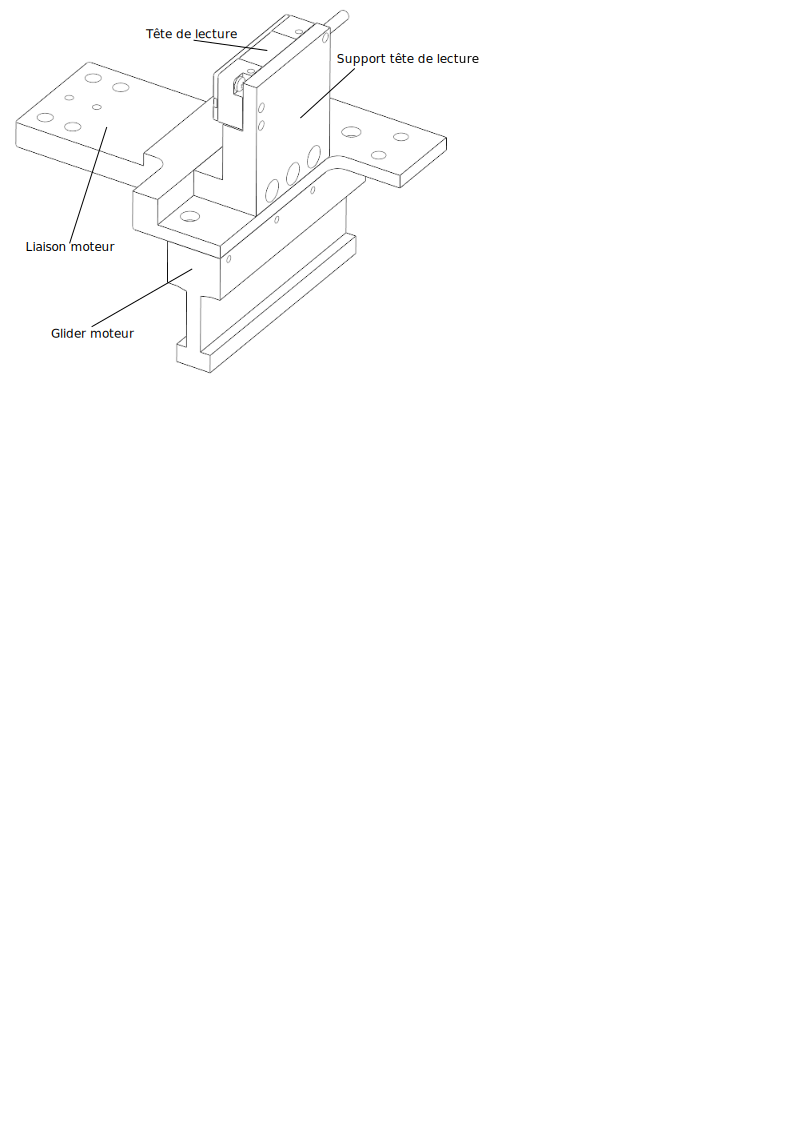
\includegraphics[width = 0.6\textwidth]{assets/figures/AssemblageMesureLineaire.png}
  \caption{Représentation du support de tête de lecture assemblée avec les pièces proches dans le système}
  \label{fig:AssMesLin}
\end{figure}

\section{Support fin de course}\label{sec:SupFinCourse}
Les capteurs de fins de course seront placés à l'arrière de la structure de chaque côté du système. Ces capteurs se fixent dans des rainures et
il faut un petit support pour pouvoir tenir le capteur et l'accrocher au système avec une vis d'où le lamage M3 nécessaire. Dans ce cas-ci, le support ne subit pas d'effort particulier
ce qui veut dire qu'il peut être fait en \acrshort{PLA} par impression 3D. Voici à quoi ressemble cette pièce.

\begin{figure}[H]
  \centering
  \includegraphics[width = 0.4\textwidth]{assets/figures/SupportFinCourse.png}
  \caption{Représentation du support de fin de course}
  \label{fig:SupFinCourse}
\end{figure}

\section{Support amortisseur}\label{sec:SupAmort}
Les amortisseurs se trouvent à l'avant du système au bout de chaque côté de la course. Leur support doit être assez épais pour pouvoir supporter
les chocs. Un trou taraudé M10 est nécessaire pour fixer l'amortisseur et deux lamages M4 permettent la fixation sur le profilé. Les deux amortisseurs
étant dans des directions opposées, il faut créer un deux support symétriques pour pouvoir les fixer. Voici l'image d'un des supports.

\begin{figure}[H]
  \centering
  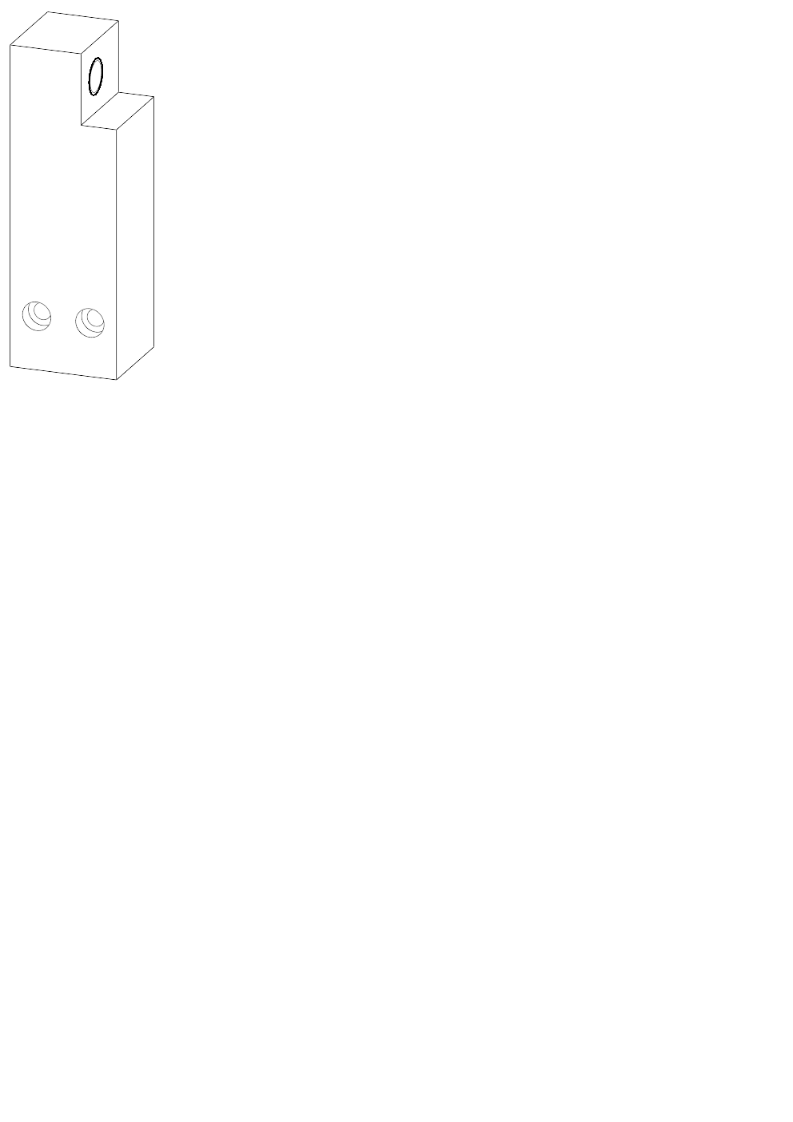
\includegraphics[width = 0.3\textwidth]{assets/figures/SupportAmortisseur.png}
  \caption{Représentation du support de l'amortisseur}
  \label{fig:SupAmort}
\end{figure}

Le placement des supports de l'amortisseur et du fin de course sur un des côtés est visible sur cette image.

\begin{figure}[H]
  \centering
  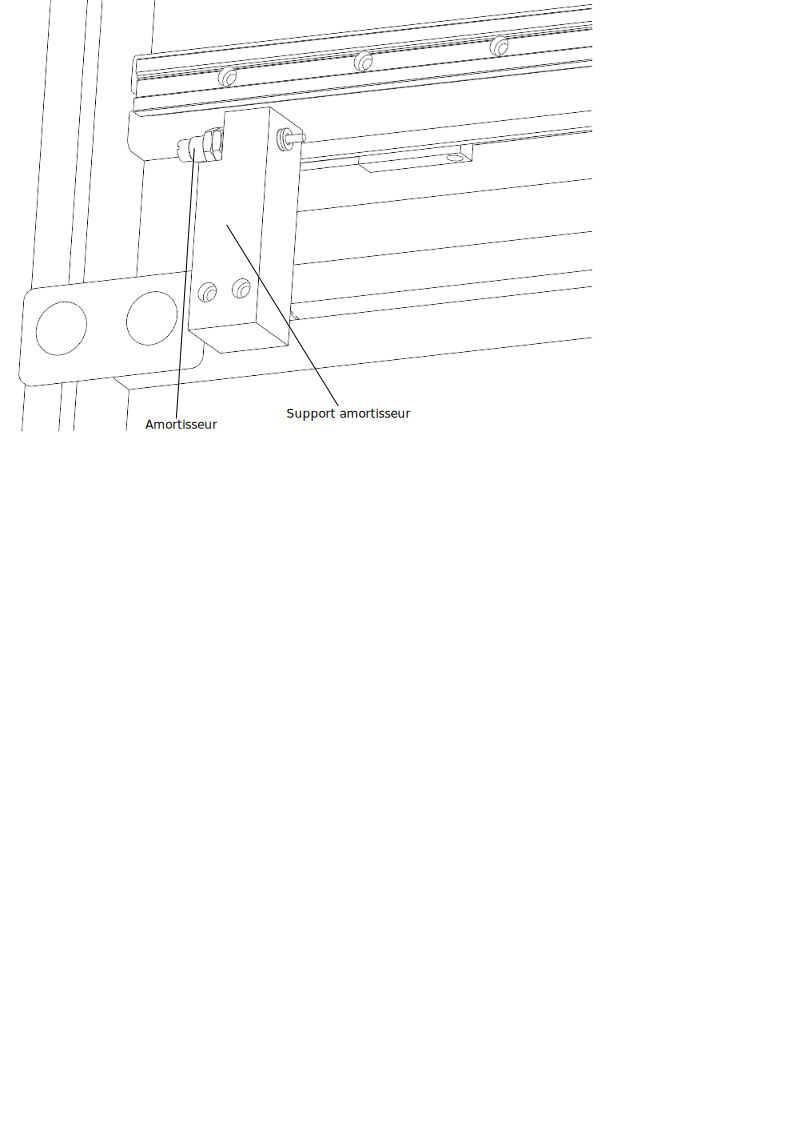
\includegraphics[width = 0.8\textwidth]{assets/figures/PlacementSupports.png}
  \caption{Représentation du placement des supports de fin de course et de l'amortisseur pour un côté}
  \label{fig:PlaceSup}
\end{figure}

\section{Partie tournante}\label{sec:PartieTour}
La partie tournante du système est composée de plusieurs pièces, dont une en \acrshort{PC}. Tout d'abord, la partie en contact direct
avec les roulements et en couplage avec l'encodeur. Cette partie est aussi attachée à une autre pièce, le couplage à la tige, à l'aide de
quatre taraudages M2. Voici à quoi elle ressemble.

\begin{figure}[H]
  \centering
  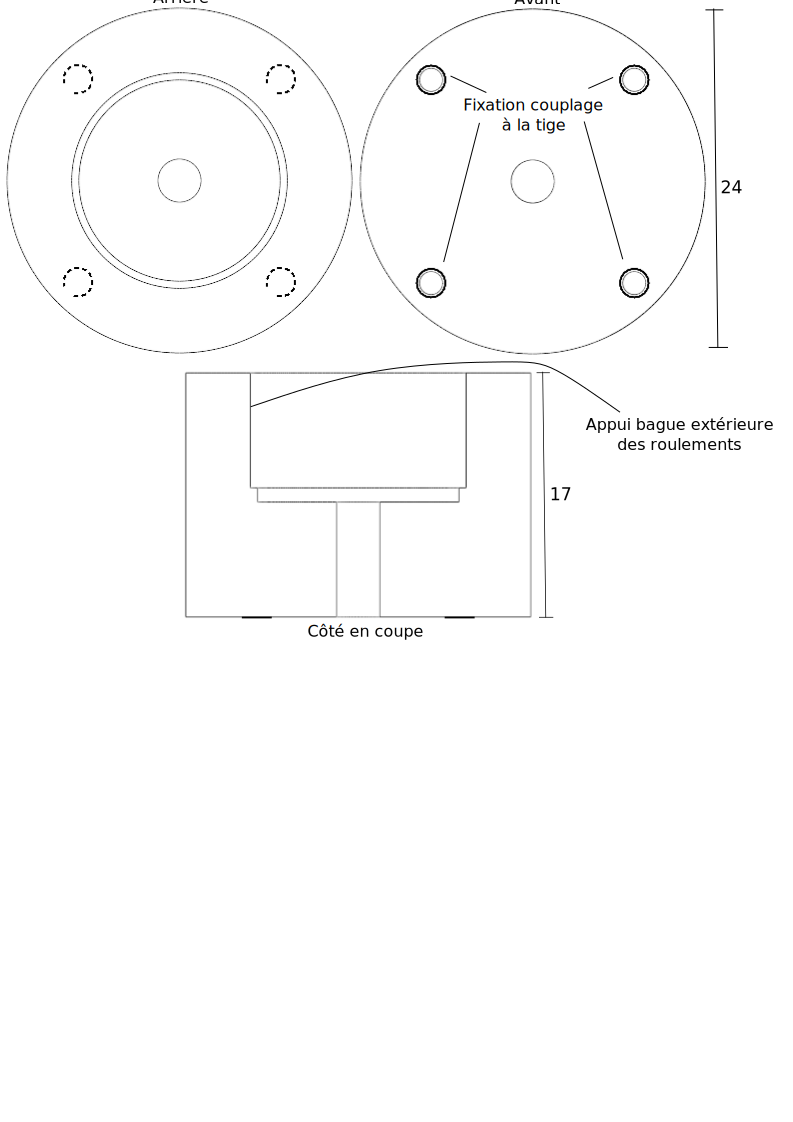
\includegraphics[width = 0.9\textwidth]{assets/figures/CouplageEncodeur.png}
  \caption{Représentation du couplage à l'encodeur}
  \label{fig:CouplEnco}
\end{figure}

La pièce de couplage à la tige qui est attachée à celle montrée sur la figure \ref{fig:CouplEnco} est en \acrshort{PC}. Elle possède donc quatre
lamages M2 pour pouvoir se visser sur la pièce précédente et aussi un perçage de 10~mm de diamètre pour venir fixer la tige par serrage.
La pièce ressemble à ceci.

\begin{figure}[H]
  \centering
  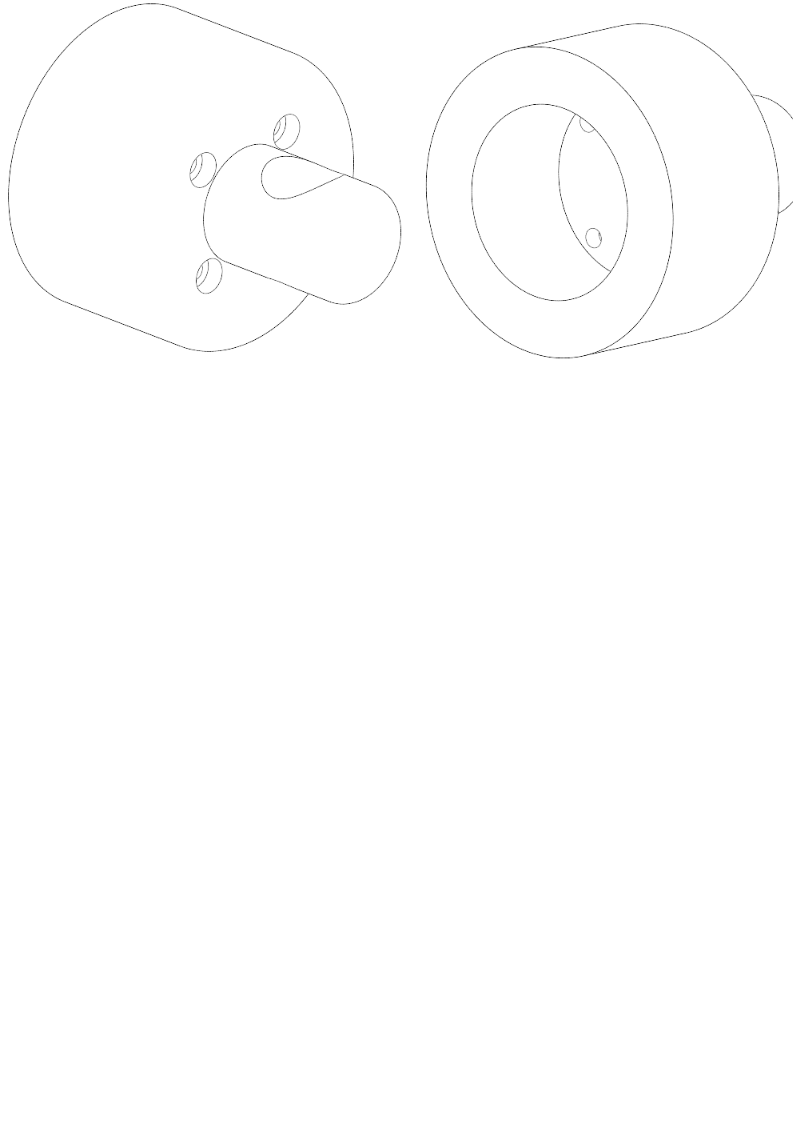
\includegraphics[width = 0.9\textwidth]{assets/figures/CouplageTige.png}
  \caption{Représentation du couplage à la tige}
  \label{fig:CouplTige}
\end{figure}

Il y a aussi la tige, elle aussi en \acrshort{PC}, qui vient se placer dans le perçage de 10~mm de la pièce précédente. La tige a donc un
diamètre lui aussi égal à 10~mm et une longueur de 420~mm. Aucune autre modification n'est apportée à la tige à part un chanfrein afin d'éviter
les arêtes coupantes.\\

L'assemblage de ces différentes pièces ainsi que de la liaison au chariot et l'encodeur donne la représentation suivante.

\begin{figure}[H]
  \centering
  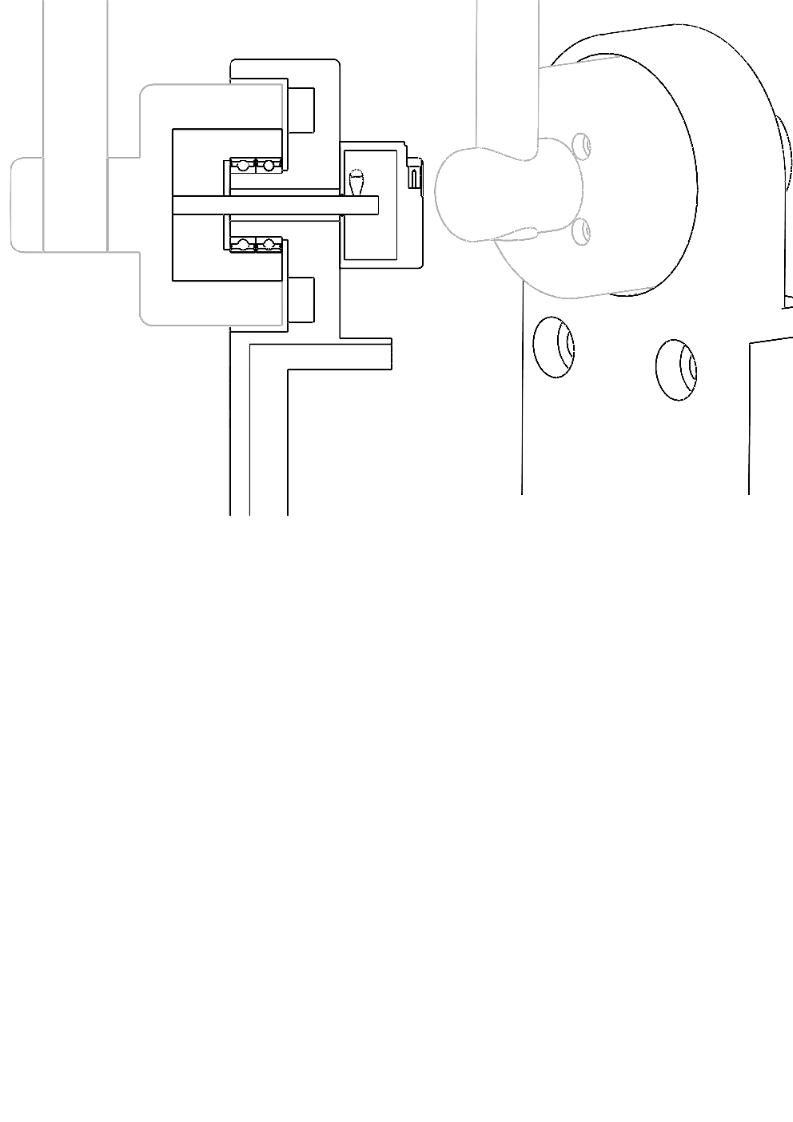
\includegraphics[width = 0.7\textwidth]{assets/figures/AssemblagePartieTournante.png}
  \caption{Représentation de l'assemblage des parties tournantes et leurs connections directes}
  \label{fig:AssPartieTour}
\end{figure}


\section{Support pour chaîne porte-câbles}\label{sec:SupChainCable}
La chaîne porte-câbles est fixée d'un côté à la liaison moteur comme précisé plus haut au chapitre \ref{sec:LiaisonMotGlid}. L'autre côté est
attaché au support pour chaîne porte-câbles qui est lui-même fixé sur un profilé. Deux passages de vis M4 sont présents pour la fixation sur
le profilé ainsi que deux autres passages de vis M6 pour la fixation de la chaîne. Il y a aussi un dégagement de matière afin de pouvoir faire
passer les câbles qui sortent de la chaîne et qui continuent plus bas vers le boîtier électrique. Cette pièce est fabriquée en tôle pliée et
nécessite un alliage d'aluminium différent, l'aluminium EN-AW 5052. Voici une image du support pour la chaîne.

\begin{figure}[H]
  \centering
  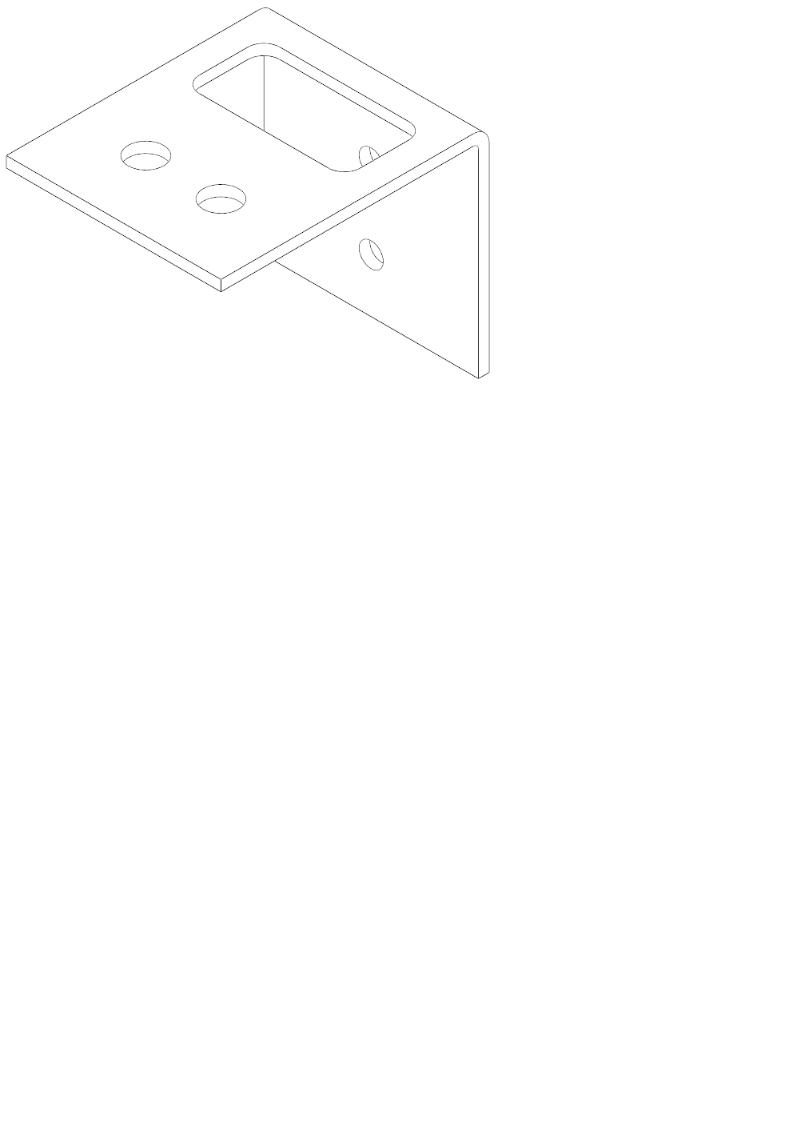
\includegraphics[width = 0.4\textwidth]{assets/figures/SupportChaineCable.png}
  \caption{Représentation du support pour la chaîne porte-câbles}
  \label{fig:SupChaineCable}
\end{figure}

\section{Plaque de passage pour moteur}\label{sec:PlaPassMot}
Afin de cacher un peu plus l'arrière du système pour le rendre présentable et aussi afin d'augmenter la rigidité du système, une plaque est placée
entre les deux profilés centraux. Les pièces faisant la liaison entre le moteur et le glider, décritent dans le chapitre \ref{sec:LiaisonMotGlid},
passent par cet endroit donc il faut découper une zone de passage pour ces pièces. Cela donne la plaque suivante.

\begin{figure}[H]
  \centering
  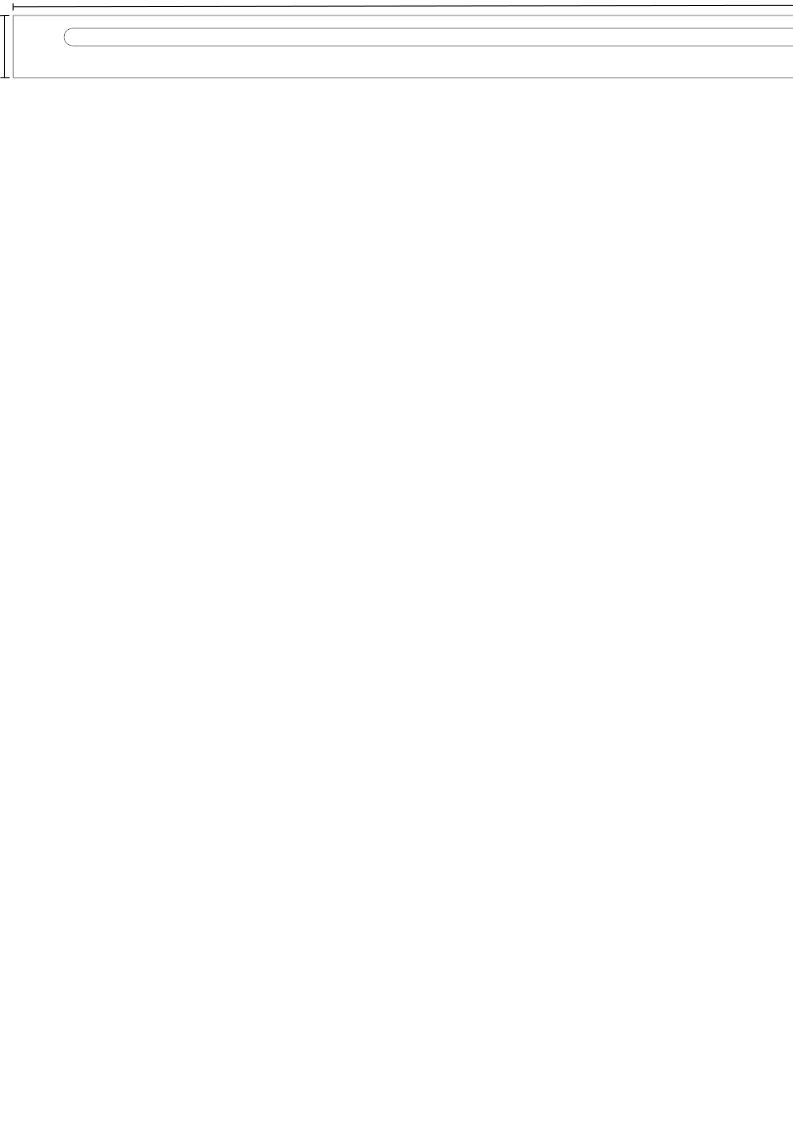
\includegraphics[width = \textwidth]{assets/figures/PlaquePassageMoteur.png}
  \caption{Représentation de la plaque centrale}
  \label{fig:PLaPassMot}
\end{figure}

\section{Assemblage mécanique complet}\label{sec:AssMecComp}
Enfin, voici l'assemblage de toutes les pièces mécaniques fabriquées avec la structure et les composants commandés vu de face et de derrière.

\begin{figure}[H]
  \centering
  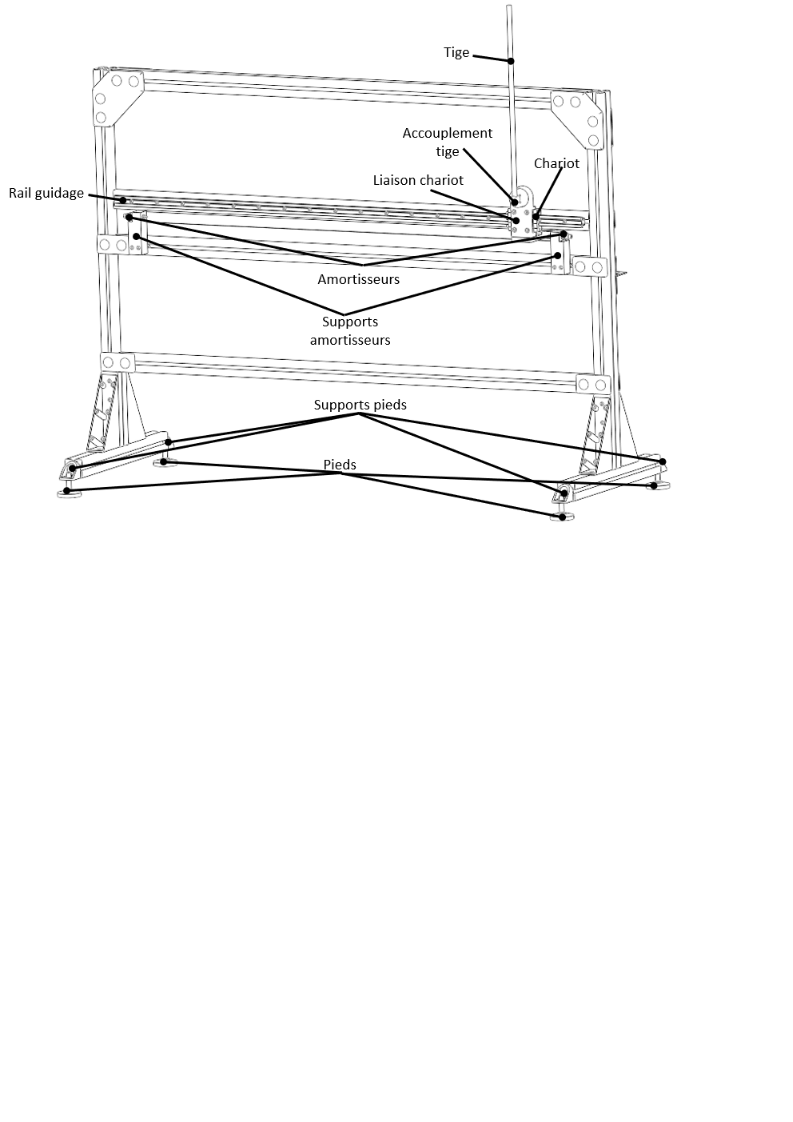
\includegraphics[width = \textwidth]{assets/figures/AssemblageCompletFace.png}
  \caption{Représentation de l'assemblage mécanique complet vu de face}
  \label{fig:AssCompFace}
\end{figure}

\begin{figure}[H]
  \centering
  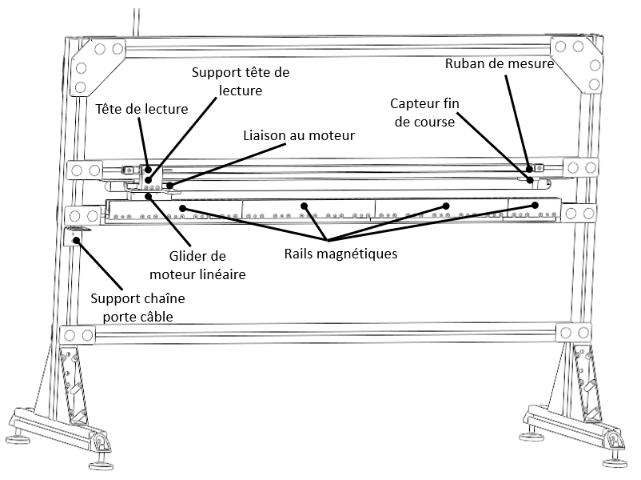
\includegraphics[width = \textwidth]{assets/figures/AssemblageCompletDerriere.png}
  \caption{Représentation de l'assemblage mécanique complet vu de derrière}
  \label{fig:AssCompDerriere}
\end{figure}